%% \documentclass[a4paper]{article}
\documentclass[12pt]{article}

%% Language and font encoding
\usepackage[english]{babel}
\usepackage[utf8x]{inputenc}
\usepackage[T1]{fontenc}

\usepackage{tgtermes} % times font

%% Sets page size and margins
\usepackage[a4paper,top=3cm,bottom=2cm,left=3cm,right=3cm,marginparwidth=1.75cm]{geometry}

%% Useful packages
\usepackage{amsmath}
\usepackage{graphicx}
\usepackage[colorinlistoftodos]{todonotes}
\usepackage[colorlinks=true, allcolors=blue]{hyperref}
\usepackage[useregional]{datetime2}
\usepackage{array}
\usepackage{tabularx}
\usepackage{natbib}
\usepackage{authblk}
\usepackage{enumitem}
\usepackage{setspace}
\usepackage{enumitem}


\renewcommand{\baselinestretch}{1.25} 






\title{Evaluation of Community Detection Algorithms}
\author{Ping-Chang Lee}
\affil{MSc in Data Science \& Statistics \\ The University of Bath}
\date{{September}{2022}}

\begin{document}
\maketitle
\pagebreak

%% Access Page 1
    
\bigbreak\bigbreak\bigbreak
\bigbreak\bigbreak\bigbreak
\bigbreak\bigbreak\bigbreak

This dissertation may be made available for consultation within the University Library and may be photocopied or lent to other libraries for the purposes of consultation.
\bigbreak\bigbreak\bigbreak
Singed: ***My Signature Here***
\pagebreak


\tableofcontents
\pagebreak

\section{Introduction}
When researchers conducting analysis on their topics, while processing data, the format of data can be form in various fashion. Table is perhaps one of the most commonly used format for data storage. However, it can be arduous for researchers to observe the relation between rows(or columns) if the data is in large scale. To ease the pain, network structure is an excellent data format that is popular among the researchers if they would like to focus on analysing data structure-wise. For analysis that is related to network structure such as study how the network change over time, visualizing the complex network, and the topic that is related to this dissertation, detecting communities within network, are called network analysis. In recent decades, the study related to network analysis has drawn the attention of scholars form various fields. Among numerous topics of network analysis, discovering the community structure of network is one of the most essential approach to learn the complicated systems that can not easily be cracked by solely conducting shallow researches\cite{1}. 

%% Add motivation/ The brief intro of the dissertation.
\bigskip

Despite there are dozens of community detection algorithms already implemented to real-world network analysis and have already granted great success in many fields \cite{2,3}, the sample networks for performance testing are often simplified and sparse. In this dissertation, the LFR benchmark graph is introduced to mock the real-world network by increasing the complexity of the network. Afterwards, a subset of community detection algorithms are applied to the artificial network. Due to the nature of algorithms, the dissertation will introduce the computation complexity and their procedures. Also, since some algorithms are iterative, the dissertation selects the best result from iterations for evaluations under different circumstances. Next, the dissertation provides a series of approaches to evaluate the partitions of algorithms. As mentioned, a network can have either high complexity or very sparse structure, there is no consistent classification yet to determine if a given partition of a network is 'good'. The dissertation particularly underline the methodology on goodness of partition and the measure of similarity between the partition of a community detection algorithm and the ground truth community partition(network that is already labeled by communities).

\section{Background}
In this section, the dissertation provides background information about the definition of network. Note that there is no fixed format of how to construct a network so far, therefore the notation used in this dissertation can be different from other papers.

\subsection{Network Structure}

The two smallest elements in network structure are vertex and edge, denoted as $v$ and $e$. Vertex is simply a node within the network, and a vertex(or a node) can contain multiple information. For instance, in social network study, each vertex represents a user, and therefore may contain some information such as phone number, physical address, searching preference, and so on.  Therefore, vertex can be treated as atom within a particle, even though vertex can take a collection of information, yet is not divisible, meaning can not be broken into smaller vertices by default. The other element is edge, an edge represent the connection between two vertices within the same network. The definition of edge is as follows:  There is an edge between vertex $v_i$ and vertex $v_j$, where $v_i$ and $v_j$ both belong to network(or a graph) $G$, if there exists an connection(or relation) between $v_i$ and $v_j$. One thing worth noticing is that an edge can be directed or weighted. For networks that contains weighted edges, the network is called weighted network; similarly, for networks that contains undirected edges, the network is called directed network. A great example of directed and weighted network is the United States Interstate Highway System(USIHS) \cite{14}, each in USIHS is usually a capital of a state or a flourish city, and the edges between these towns are highways with precise length in kilometers. Beside these popular types of network, there are also other networks with interesting properties; however, to focus on the purpose of this dissertation, further study can be done by reading the book, Introduction to Graph Theory Fourth edition \cite{15}.

\bigbreak

In general, there are two components that construct a network. A network(or a graph) G is composed by V and E, where V is the vertex(node) set containing all the vertices that belongs to the network and E is the edge(relation) set containing all the edge between vertices if two are connected. The mathematical expression of network is defined as: $G = \{V, E\}$. Further properties can be added to the network if the network is weighted or directed. 

\bigbreak

When conducting analysis on a network, forming raw data into network structure can be beneficial in data storage and has lower computation complexity in particular cases comparing to other relational structure \cite{6}. In the field of database management system, there are three practical approaches to store network structure data. For the sake for clarity, assume we have a small undirected and unweighted network containing four vertices, namely 1, 2, 3, and 4, and four edges, 1 connects to 2, 1 connect to 3, 2 connects to 3, and 3 connects to 4. Mathematically, $G = \{V, E\} \text{,where }V=\{1,2,3,4\}\text{ and }E=\{(1,2),(1,3),(2,3),(3,4)\}$. The visualization of the graph is shown in figure \ref{fig:fig_1} .

%% Finish the graphical data structure
\begin{enumerate}[label=(\roman*)]
\item Edge List:
\item Adjacency Matrix:
\item Map: 
\end{enumerate}


\bigskip
\begin{figure}
    \centering
    \begin{minipage}{0.45\textwidth}
        \centering
        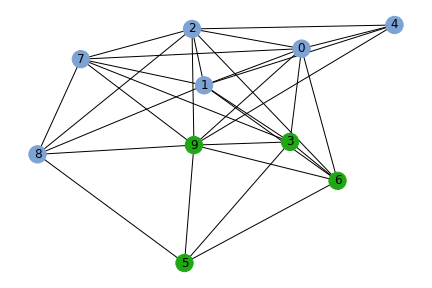
\includegraphics[width=0.9\textwidth]{fig_1.png} % first figure itself
        \caption{\label{fig:fig_1} A visualization of a network with 4 vertices and 4 edges.}
    \end{minipage}\hfill
    \begin{minipage}{0.45\textwidth}
        \centering
        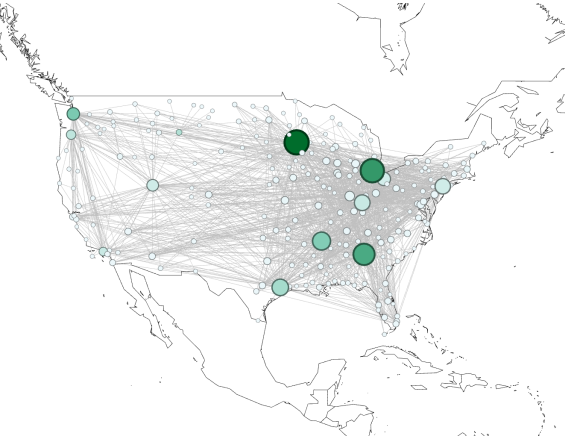
\includegraphics[width=0.9\textwidth]{fig_2.png} % second figure itself
        \caption{\label{fig:fig_2}A network with unique ID and color labels. In this network, there are two communities whose nodes are either colored in sky blue or in grass green.}
    \end{minipage}
\end{figure}


\subsection{Community}

In network analysis, community in a network often refers to a group of vertex that has closer relation comparing to other vertices that are not in the same group. In order to fit the goals of this dissertation, the label function L is add to the network, that is $G = \{V,E,L\}$. $L(v_i) = c_j$ indicates vertex $v_i$ belongs to community with label of $c_j$. With the definition of label stated previously, the community $C_i$ can be defined as $C_i = \{ L(v) = c_i \text{, } \forall v \in V \}$. Furthermore, given a partitioned network with n communities, let $C_i$ be the community with a label of $c_i$, then $\bigcup_{1 \leq i \leq n} C_i \subseteq V(G)$.  To simplify the complexity of the context, in this dissertation, no vertex will be assigned to multiple communities, that is $\forall C_i,\ C_j \text{, } i \neq j$, $C_i \cap C_j = \phi$. Depending on the content of network, such as social network, chemical network, and ecosystem network, the definition of forming a community may vary. Furthermore, if given a weight network such as a geographical network, we can intuitively determine if vertices can be grouped into a community by taking their distance(weight of edges) into consideration. Directed network can also be partitioned into communities if the community detection is designed carefully with the help of linear algebra and information theory\cite{4}. Without doubt, there are networks that has no intention of creating communities such as random graphs or Barabási–Albert model\cite{5}; researchers can still apply community detection algorithms to unveil the latent structure from these networks.

\section{Goodness of Partition}

Intuitively, to examine if a partition is 'good' or not, researchers should measure following two properties: 
\begin{enumerate}[label=(\alph*)]
\item Tightness: Vertices within the same community should have strong relation.
\item Sparsity: Communities should have weak relation mutually.
\end{enumerate}[label=(\alph*)]

In this section, a number of approaches will be introduced to evaluate the partition considering the properties mentioned above. Other additional properties such as betweeness, conductivity, and modularity are often take into consideration for better understanding of specific types of real-world network\cite{7,8}; some additional properties will also be explained in this section.

\subsection{Performance Evaluation}
A good partition should have high tightness intra-community-wise and strong trait of sparsity inter-community-wise. Given a undirected partitioned network, a performance function $P(G)$ is defined as
$$P(G) = \frac{\text{edge of intra-community} + \text{non-edge of inter-community}}{\text{total potential edges}}$$
$$=\frac{|E_{intra}| + [n*(n-1) - |E_{intra}| - |E_{inter}|]}{n*(n-1)/2}$$
$$=2*\left[ 1 - \frac{ |E_{inter}| } { n*\left( n-1 \right) }  \right],$$
where G is a partitioned network, $E_{intra}$ is the set of edges lie within communities, $E_{inter}$ is the set of edges connecting vertices between two different communities. 

\bigbreak

After a series of rearrangement, it is not difficult to observe that a network has smaller set of inter-community edges can leads to higher value of $P(G)$(better performance)\cite{7}. In the aspect of algorithm complexity analysis, the time complexity of performance evaluation is in $O(E)$, where E is the edge set; with linear time complexity, researchers can conduct faster initial evaluation comparing to other advanced evaluation procedures.

\subsection{Mean Square Error}
For networks with coordinates provided, take geographical network or cosmic network for instance \cite{9,10}, computing the mean square error(MSE) evaluation can give us an idea if a partition is good. A demonstration of geographical network is shown in figure \ref{fig:fig_3}. The quality function of MSE evaluation is defined as follows:
    $$Q(G) = \sum_{i}^{k}\sum_{j}^{n} M_{i j} * |v_{j} - \bar{v}_{i}|^{2},$$
where G is a partitioned network, k is the total number of communities in a partition, n is the count of the vertices of network $G$, $M$ is a k by n communities matrix, \[
  M_{ij} = 
  \begin{cases}
    1, &  v_{j} \in C_i\\
    0, & \text{otherwise}
  \end{cases}
\]
, and $\bar{v}_{i}$ is the arithmetic center of $C_i$. 

\bigbreak

This evaluation is relatively straightforward; if given a well-partitioned network, it is expected vertices within the same community cluster densely and surrounds the center of the community; such behavior results in mean square error within every community approaches to zero. The computation complexity of MSE evaluation is in $O(C*V)$, the computing time can be reduced by pre-allocating vertices into a collection of set distributed by the partition.

\begin{figure}
\centering
\includegraphics[width=0.6\textwidth]{fig_3.png}

\caption{\label{fig:fig_3}An airline flight network of the United States of America\cite{11}.}
\end{figure}

\subsection{Modularity}

This evaluation method is first introduced by Blondel in 2008 \cite{12}. When tackling with a humongous and complex network, a fast and approximated evaluation algorithm is necessary for time and resource efficiency. In this end, the modularity evaluation stands out to do this job. The modularity function \cite{13} can be written as follows:
\begin{equation}\label{eq:modularity}
Q = \sum_{i=1}^c \left[  \frac{e_i}{m} - \left( \frac{deg_i}{2m} \right)^2  \right],
\end{equation}
where $c$ is the count of communities, $e_i$ is the count of edges within the community $i$, $m$ is the count of the edge of the network, and $deg_i$ is the total degree of vertices within community $i$. The logic of modularity is similar to hypothesis testing: an alternative model and a null model is defined for comparison. The first term of equation \eqref{eq:modularity}, which is the alternative model in this case, is the fraction of edges within a community to total edges of the network; and the second term, the null model, is the expected fraction based on the assumption that edges are randomly connected.

\bigbreak

Given an undirected and unweighted network, the value of modularity lies in range $[-1, 1]$. If the edges within a community exceed the expected count of edges, the first term will be greater than the second term, leading the $Q$ value of that community become positive. This implies that the edges inside the community are averagely concentrated. As author stated in the original paper \cite{12}, implementing modularity to examine the partition is not the only usage. The modularity function is as well suitable for partition optimization for  networks. The community detection algorithms that import modularity optimization, such as Louvain method, will be discussed in the latter section.

\bigbreak

Despite the time complexity of computing modularity is in $O(n*log n)$, which is faster comparing to other meta partition evaluations \cite{2, 12}, the modularity evaluation is not capable of detecting small communities. The defect is inevitable due to the nature of the null model defined previously, the modularity only considers the structure of communities under global scope; as for local structure evaluation, the modularity ignores heterogeneity of sizes between communities \cite{13}. In real world applications \cite{9, 10}, the modularity evaluation may suggest small communities should be merged into a greater community, causing false estimation of structure and count of communities. Such over-merging behavior is called resolution limit \cite{13}.

%% (Done)Read more about modularity and it's concept
%% (Done)Read resolution limit (over-merging) 

\subsection{Normalized Mutual Information}

%% Work on NMI chapter intro
%% In Evaluation of Community Detection Methods, NMI is counter-intuitive and unreasonable due to lack of consideration of local community strucure
%% Introduce new NMI indicator: adding the summation of v_partition/v_true as coefficients into orginal NMI model(Treat all communities equally to reduce size discrepancy)
%% (Done)Read page 3 "Evaluation of Community Detection Methods"

\pagebreak
\begin{thebibliography}{100}

\bibitem{1}
  
    \textit{Community detection algorithms: A comparative analysis},
    Lancichinetti, A. and Fortunato, S.,2009.
    1986.
  
\bibitem{2}
    \textit{Parallel Protein Community Detection in
    Large-scale PPI Networks Based on
    Multi-source Learning}
    J. Chen, K. Li, K. Bilal, A. A. Metwally, K. Li, and P. S. Yu,
    2018
    
\bibitem{3}
    \textit{Community detection in Social Media. Data Mining and Knowledge Discovery}
    Papadopoulos, S., Kompatsiaris, Y., Vakali, A. and Spyridonos, P.,
    2011
    
\bibitem{4}
    \textit{Quantitative methods for ecological network analysis. Computational Biology and Chemistry}
    Ulanowicz, R.E.,
    2004
    
\bibitem{5}
    \textit{tatistical mechanics of complex networks. Reviews of Modern Physics}
    Albert, R. and Barabási, A.-L.,
    2002
    
\bibitem{6}
    \textit{Comparison of Graph Databases and Relational Databases When Handling Large-Scale Social Data}
    Chen, Yaowen,
    2016
    
\bibitem{7}
    \textit{Community detection in graphs}
    Fortunato, S.,
    2010
    
\bibitem{8}
    \textit{Community structure in social and biological networks}
    Girvan, M. and Newman, M.E.J.,
    2002
    
\bibitem{9}
    \textit{Network analysis of the COSMOS galaxy field}
    de Regt, R., Apunevych, S., von Ferber, C., Holovatch, Y. and Novosyadlyj, B,
    2018
    
\bibitem{10}
    \textit{Evaluation of Community Detection Methods}
    Liu, X., Cheng, H.-M. and Zhang, Z.-Y,
    2019
    
\bibitem{11}
    \textit{An Introduction of Gephi}
    2017

\bibitem{12}
    \textit{Fast unfolding of communities in large networks}
    Blondel, V.D., Guillaume, J.-L., Lambiotte, R. and Lefebvre, E
    2008
    
\bibitem{13}
    \textit{Resolution limit in community detection}
    Fortunato, S. and Barthelemy, M.,
    2006

\bibitem{14}
	{Federal-Aid Highway Act of 1956: Creating The Interstate System}
	Richard F. Weingroff,
    1996
    
   \bibitem{15}
   	{Introduction to Graph Theory Fourth edition }
    Robin J. Wilson,
    1996
        
\end{thebibliography}

\end{document}